%%%%%%%%%%%%%%%%%%%%%%%%%%%%%%%%%%%%%
%%%%% PHYS305 Assignment 8
%%%%% Zachary Martin
%%%%% 25 March 2019
%%%%%%%%%%%%%%%%%%%%%%%%%%%%%%%%%%%%%

\documentclass[aps,prl,twocolumn,superscriptaddress]{revtex4-1}

\usepackage{graphicx}  % this is the up-to-date package for all figures
\graphicspath{{pictures/}} 	% Set Graphics Path
\usepackage{siunitx} % Scientific Notation and Units
\sisetup{separate-uncertainty}
\DeclareSIUnit\mph{mph}
\usepackage{amsmath, amssymb, gensymb, mathtools, bm, bigints} 	% Mathematical Tools
\usepackage{verbatim}  % for the comment environment
\usepackage{color}
% \usepackage{arydshln} % Dashed lines in table

% For inserting code snippets
\usepackage{listings}
\usepackage{xcolor}
\lstset { %
    language=C++,
    backgroundcolor=\color{black!5}, % set backgroundcolor
    basicstyle=\footnotesize,% basic font setting
}

% Shortcut Commands
\newcommand{\paren}[1]{\left( #1 \right)} 	% Parentheses for complicated expressions
\newcommand{\bparen}[1]{\left[ #1 \right]}	% Bracket parentheses for complicated expressions
\newcommand{\cmod}[1]{\left| #1 \right|}	% Mod or Absolute value

\bibliographystyle{apsrev}

% these are some custom control of the page size and margins
% \topmargin= 0.2in  % these 1st two may be needed for some computers
\textheight=9in
\textwidth=6.5in
% these next two lines give us centered text
\oddsidemargin=0cm
\evensidemargin=0cm

%\begin{figure}[htbp]
%  	\begin{center}
% 		\includegraphics[scale=0.3]{.png}
%  		\caption{}
%  		\label{gr:}
% 	\end{center}
%\end{figure}

\begin{document}

% Title Contents
\title{PHYS 305 Assignment 8: Analyzing Drag in Projectile Motion of Baseball Home-Runs via Fourth-Order Runge-Kutta Methods.}
\author{Zachary Martin}
\affiliation{University of Hawaii at Manoa}
\date{27 March 2019}

\begin{abstract}
We examine the effects of air resistance on a home-run struck baseball by employing the fourth order Runge-Kutta method to numerically solve the equations of motion. We find that drag alters the resulting range by about a $43$\% difference and that the angle of maximum range changes from the known $\SI{45}{\degree}$ to $\SI{40}{\degree}$. Drag is also found to create asymmetrical behaviors in the range and angles. The effects on the properties of the air and wind are also examined and found to have similar effects for specific ranges of values.
\end{abstract}

\maketitle

\section{Introduction and Overview}
Projectile motion is one of the fundamental problems in beginner-level physics which can be described through the simple kinematic equations of motion. The equation of motion for a two dimensional projectile launched at an angle $0 \leqslant \theta_0 \leqslant 90$ at some velocity $v_0$ is
\begin{equation}
\frac{d^2\bm{x}}{dt^2} = -\bm{g} \label{eq:dvdttrue}
\end{equation}
without air resistance and on Earth with gravitational acceleration $\bm{g} = g\bm{\hat{y}}$. The analytic solution, obtained by integrating, is
\begin{equation}
\bm{x} = \bm{v_0}t - \frac{1}{2}\bm{g}t^2 ~. \label{eq:truesol}
\end{equation}
Separating the components, we can obtain a function of the 2D trajectory,
\begin{equation}
y =  x\tan\theta - \frac{g x^2}{2 v_0^2\cos^2\theta} ~. \label{eq:trajtrue}
\end{equation}
The range $R(\theta)$ can then be found to be
\begin{equation}
R(\theta) = \frac{v_0^2 \sin 2\theta}{g} ~,\label{eq:range}
\end{equation}
which has a maximum value at $\theta_{\text{max}} = \SI{45}{\degree}$.
We now wish to see the effect of air resistance on the trajectory.

\subsection{Projectile Motion with Air Resistance}
There are many ways that air resistance can affect a projectile. The three main types are lift induced, parasitic, and wave drag which differ by the different behaviors of the air \cite{drag}. For high velocities, these types of drag are calculated with the quadratic drag equation,
\begin{align}
\bm{F_D} &= \frac{1}{2}C_DA\rho(h)\bm{v}^2\bm{\hat{v}} \label{eq:drag} \\
&= b\cmod{\bm{v_{\text{app}}}}\bm{v_{\text{app}}} ~, \label{eq:drag2} 
\end{align}
where $C_D$ is a drag coefficient, $A$ is the cross sectional area of the object. We consider a baseball ($C_D = 0.3$, $A = 0.5 \pi (\SI{0.0369}{\m})^2$, $m = \SI{0.145}{\kg}$) being struck at mean home-run velocity $v_0 = \SI{45.2}{\m\per\s}$. We have also defined
\begin{align}
b &= \frac{1}{2}C_DA\rho(h) \label{eq:b} \\
\bm{v_{\text{app}}} &= \bm{v} - \bm{W} ~. \label{eq:vapp}
\end{align}
Here, $\bm{W}$ represents any present wind. We have that the air density $\rho(h)$ can be written as \cite{Laulima}
\begin{equation}
\rho(h) = \rho_0 e^{-h/h_0} ~. \label{eq:rho}
\end{equation}
where $\rho_0$ and $h_0$ are parameters that depend on the location on Earth. At sea level, $\rho_0 = \SI{1.22}{\kg\per\m\cubed}$ and for heights below $\SI{3}{\km}$, we can use $h_0 = \SI{8300}{\m}$. With this equation for the force of drag, we can derive the equations of motion
\begin{align}
\frac{d\bm{x}}{dt} &= \bm{v} \label{eq:dxdt} \\
\frac{d\bm{v}}{dt} &= -\bm{g} - \frac{b}{m}\cmod{\bm{v_{\text{app}}}}\bm{v_{\text{app}}} ~. \label{eq:dvdt}
\end{align}
Not only do are these coupled differential equations, but Equation \ref{eq:dvdt} is a second order differential equation. We will avoid the analytic solution, and use a numerical approach.

\section{The Computational Problem}

\begin{figure}[htbp]
  	\begin{center}
 		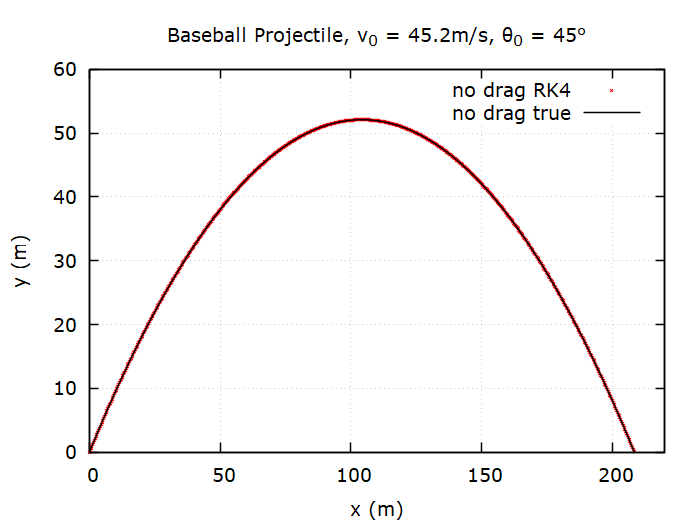
\includegraphics[scale=0.3]{projcompare.png}
  		\caption{A comparison of the true projectile trajectory curve without drag and the RK4 results.}
  		\label{gr:projfit}
 	\end{center}
\end{figure}

\begin{figure}[htbp]
  	\begin{center}
 		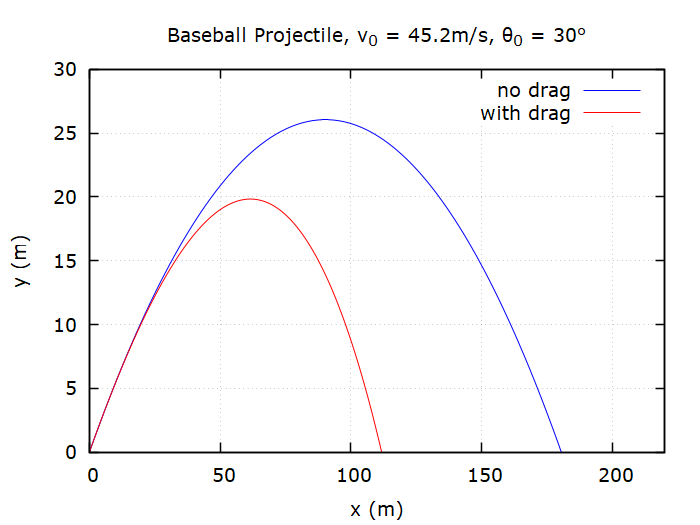
\includegraphics[scale=0.3]{proj30.png}
 		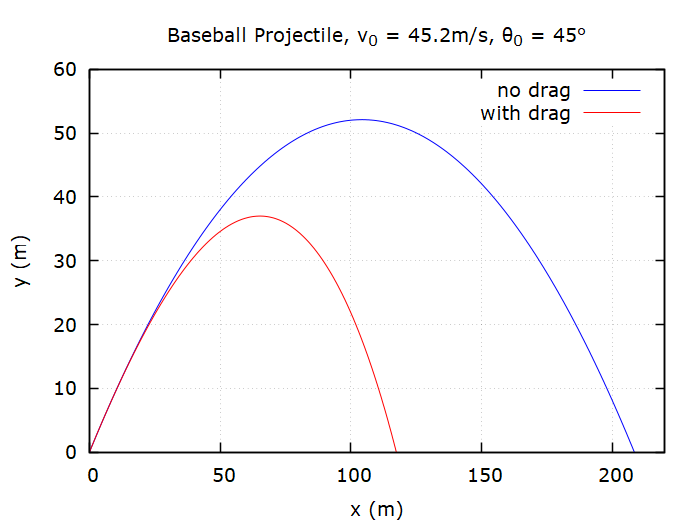
\includegraphics[scale=0.3]{proj45.png}
 		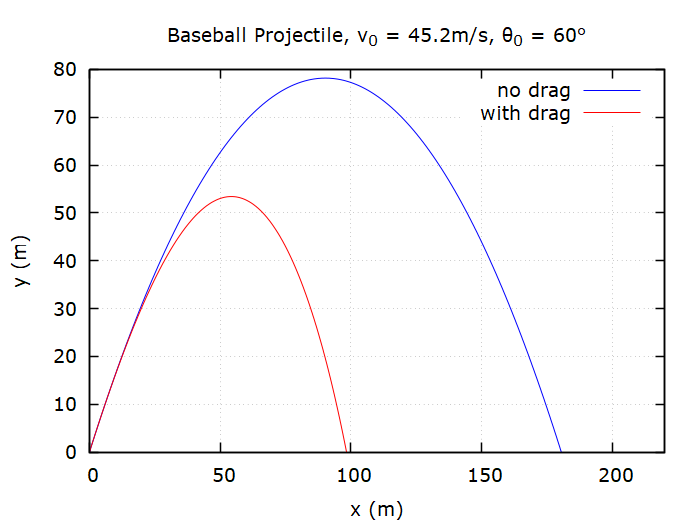
\includegraphics[scale=0.3]{proj60.png}
  		\caption{The baseball trajectories with (red) and without (blue) drag for trajectory angles 30, 45, and 60 at home-run velocity. The curve with drag is asymmetrical and is smaller than the curve without drag, as we would expect.}
  		\label{gr:proj}
 	\end{center}
\end{figure}

The coupled differential equations \ref{eq:dxdt} and \ref{eq:dvdt} can be solved numerically with a fourth order Runge-Kutta Method (RK4). The method builds upon the ideas of Euler's Method, treating each step as a linear approximation, but adds up to fourth-order correction terms to account for the change in slope at each step \cite{RK4}. This involves multiple tedious calculations, but can be handled simply using computational methods. By creating a function which determines the correction term, we can simply call to it in our numerical program to solve the differential equation. 

\begin{lstlisting}
vec3 f_x(double t, vec3 x, vec3 v)
{
return(v);
}

vec3 f_v(double t, vec3 x, vec3 v)
{
double  g=9.8, m=0.145, r=0.0369;
double b = 0.5*M_PI*pow(r,2.0)*dragc(x.z);
//b = 0.0; //(un)comment - on/off drag
vec3 W;	// wind
  W.x = 0.0; W.y = 0.0; W.z = 0.0;
vec3 vapp = vec3sum(v, W);

vec3 retval;
  retval.x = -(b/m)*vec3mag(vapp)*vapp.x;
  retval.y = -(b/m)*vec3mag(vapp)*vapp.y;
  retval.z = -g-(b/m)*vec3mag(vapp)*vapp.z;
return(retval);
}

double dragc(double H)
{
double Cd = 0.30, rho0 = 1.22, h0 = 8300.;
double Cdrho = Cd*rho0*exp(-H/h0);
return(Cdrho);
\end{lstlisting}
Here, we have Equation \ref{eq:dxdt} as $f\_x$ and Equation \ref{eq:dvdt} as $f\_v$. Using the RK4 correction terms, we can now iterate through steps of time to calculate the values of $\bm{x}$ and $\bm{v}$:
\begin{lstlisting}
for(t=t0; t<Tmax; t+= dt){
xt = vec3sum( xtold ,
  vecFRK4xv(0,f_x,f_v,t,xtold,vtold,dt) );
vt = vec3sum( vtold ,
  vecFRK4xv(1,f_x,f_v,t,xtold,vtold,dt) );
xtold = xt;
vtold = vt;
}
\end{lstlisting}
From Figure \ref{gr:projfit}, we can see that the RK4 method is successful in recreating the results of the true projectile motion with no air resistance, which we calculated in the Introduction.
We can now simulate the results for multiple angles and compare how drag changes these results.

\section{Results and Graphs}

\begin{figure}[htbp]
  	\begin{center}
 		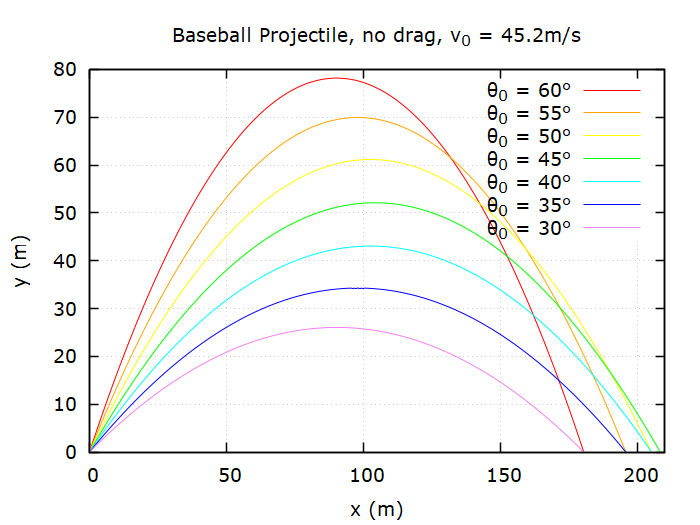
\includegraphics[scale=0.3]{projnodrag.png}
 		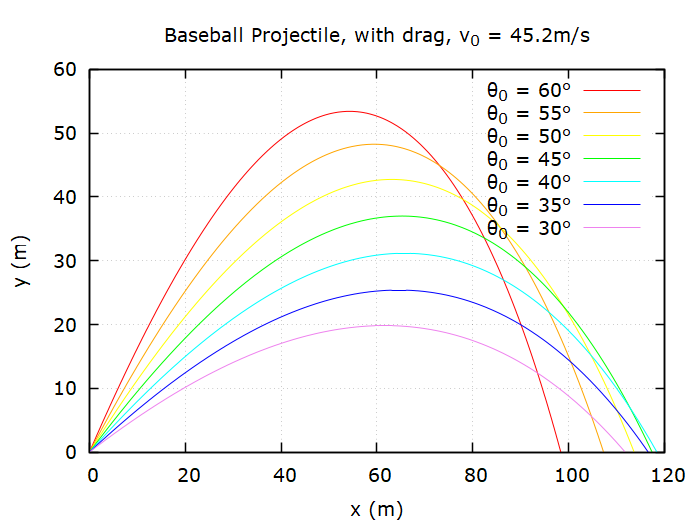
\includegraphics[scale=0.3]{projwdrag.png}
  		\caption{The trajectories of a home-run struck baseball with (bottom) and without (top) drag for initial launch angles of $\SI{30}{\degree}$ to $\SI{60}{\degree}$ at $\SI{5}{\degree}$ increments. Notice how the range of distances for the curves with drag are much smaller than the range of distances for the curves without drag. For a better look at the values of the range for each curve, see Figure \ref{gr:avr}.}
  		\label{gr:projdrag}
 	\end{center}
\end{figure}

\begin{figure}[htbp]
  	\begin{center}
 		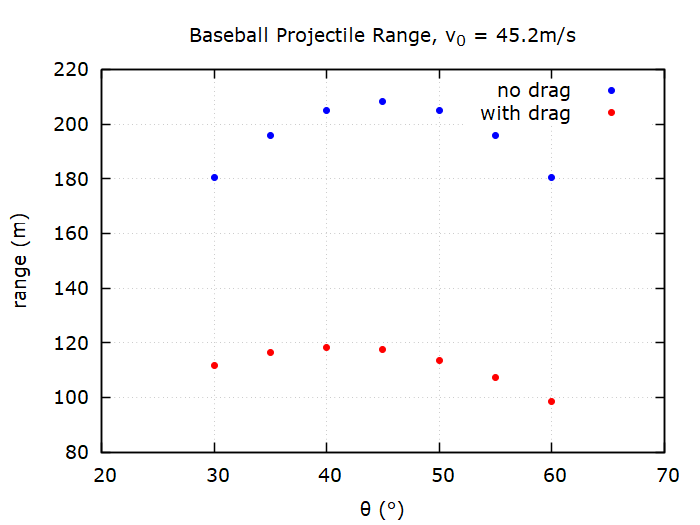
\includegraphics[scale=0.3]{avr.png}
  		\caption{The values of trajectory ranges for varying initial velocity angles. We can see that for no drag, the angle of maximum range is $\theta_{\text{max}} = \SI{45}{\degree}$ as we expect \cite{ang}. With drag, the angle of maximum range is shown to be $\theta_{\text{max}} \approx \SI{40}{\degree}$. Note that the relationship is not symmetrical about the maximum for the curve with drag.}
  		\label{gr:avr}
 	\end{center}
\end{figure}

\begin{figure}[htbp]
  	\begin{center}
 		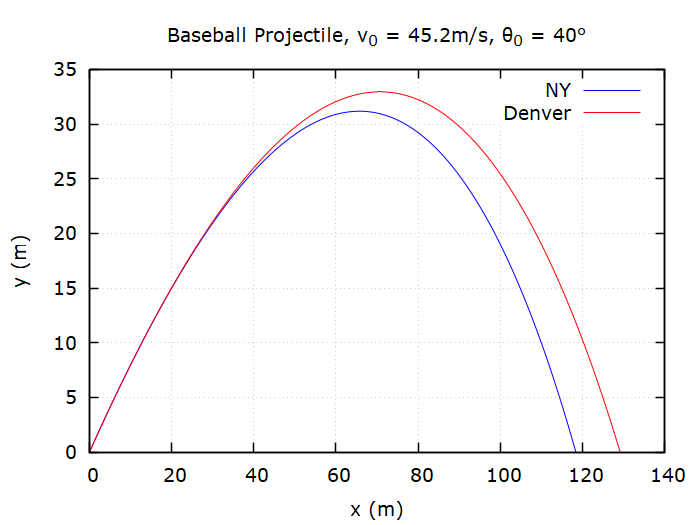
\includegraphics[scale=0.3]{NYvDen.png}
 		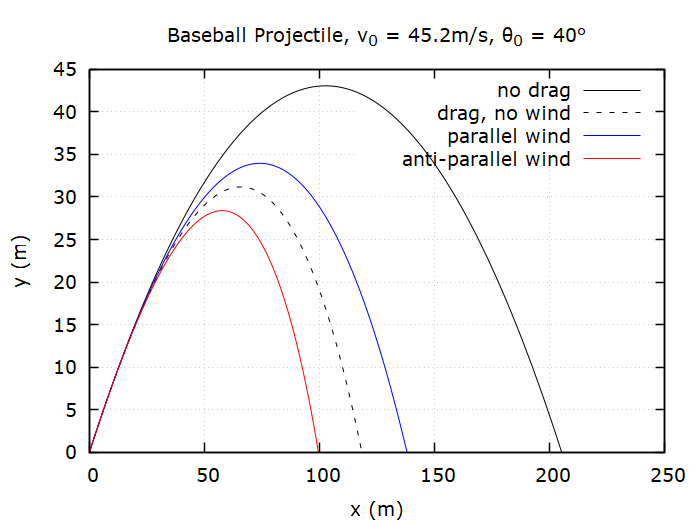
\includegraphics[scale=0.3]{wind.png}
  		\caption{The trajectory with varied density (top) and wind (bottom). The air density at sea-level (New York) is $\rho_0 = \SI{1.22}{\kg\per\m\cubed}$ and at $\SI{1600}{\m}$ (Denver) is $\rho_0 = \SI{1.056}{\kg\per\m\cubed}$ \cite{air}. The wind velocity was chosen to be $\SI{15}{\mph} = \SI{6.7056}{\m\per\s}$ either parallel or anti-parallel to the velocity of the baseball. These were all chosen to be at the angle of maximum range for drag, found from Figure \ref{gr:avr}.}
  		\label{gr:vary}
 	\end{center}
\end{figure}

\section{Discussion and Analysis}
The figures in the Results section show clearly how the presence of drag changes the results of the projectile motion. In all figures, the resulting range is significantly reduced to around $50$ to $65$ percent the original range. Notice how the curve with drag in Figure \ref{gr:proj} remains the same as the curve without drag at short distances, and afterwards is completely under. This is exactly what we would expect to happen as a result of drag. 

We can see the different results for the range at different angles in Figure \ref{gr:avr}. We get the expected maximum range angle of $\SI{45}{\degree}$ for the case without drag. When drag is present, it appears to be that the maximum range angle decreases to $\SI{40}{\degree}$ for this situation. This makes sense because the ball needs to use most of its velocity to move forward rather than upward to reach a farther distance.

There is also a slight asymmetrical behavior of the results with drag. This is shown clearly in Figures \ref{gr:projdrag} and \ref{gr:avr}. Without drag, the angles above and below the maximum range angle give the same result, whereas with drag, the range is still better for angles slightly above $\theta_{\text{max}}$ than for angles slightly below. The range does however decrease greatly once above $\SI{50}{\degree}$.

In Figure \ref{gr:vary}, we can see how changing location (air density) or how adding wind will affect the results. In Denver, we see that the lower air density results in a greater range. This makes sense, since there are less air molecules per cross sectional area to take away momentum from the baseball. For $\SI{15}{\mph}$ winds either parallel or anti-parallel to the velocity of the ball, the difference is quite similar to the difference from changing air density. The effect of wind is however stronger by a bit. Note that the effect of changing air density is bounded by the curve with no drag (zero air density), but the wind can increase without bound (theoretically) and so has a much more significant effect. But it does appear that the effects do have a slight agreement in some range of values. The effect of the shape of the curve seems negligible, so attempting to identify the cause of the difference given the results would not be an easy task, which I believe is unexpected.

\section{Conclusions}
It is clear that air resistance plays a significant role in the results of a system, such as projectile motion. Despite the complexity it may add to analytic solutions, it cannot be ignored in real world calculations. Luckily, this simulation has shown the power of computational methods in solving such complex equations.

For a home-run struck baseball, the maximum range and angle of maximum range are $R = \SI{208.39}{\m}$ and $\theta = \SI{45}{\degree}$ without the presence of drag. With drag, the maximum range and corresponding angle are $R = \SI{118.57}{\m}$ and $\theta = \SI{40}{\degree}$, about a $43$\% difference in range and $11$\% difference in angle. These are significant differences in results that it is clear air resistance cannot be ignored.

\section*{Acknowledgments}
\setlength{\parindent}{0cm}

\bibliographystyle{aipauth4-1}
\bibliography{bib8}



\end{document}